% Copyright (C) 2010,2011,2012,2013 The ESPResSo project
% Copyright (C) 2011 Florian Fahrenberger
% Copyright (C) 2004 Igor Pasichnyk
% Copyright (C) 2002,2003,2004,2005,2006,2007,2008,2009,2010 
%   Max-Planck-Institute for Polymer Research, Theory Group
%  
% This file is part of ESPResSo.
%   
% ESPResSo is free software: you can redistribute it and/or modify it
% under the terms of the GNU General Public License as published by the
% Free Software Foundation, either version 3 of the License, or (at your
% option) any later version.
%  
% ESPResSo is distributed in the hope that it will be useful, but
% WITHOUT ANY WARRANTY; without even the implied warranty of
% MERCHANTABILITY or FITNESS FOR A PARTICULAR PURPOSE.  See the GNU
% General Public License for more details.
%  
% You should have received a copy of the GNU General Public License
% along with this program.  If not, see <http://www.gnu.org/licenses/>.
%
\chapter{Maxwell Equations Molecular Dynamics (MEMD)}
\label{sec:MEMD}

In this chapter, we want to give a more thorough introduction to the
MEMD (or ``Maggs'') algorithm for the calculation of Coulomb
interactions that is implemented in \es{}. For an even more detailed
description, we refer to the publications \cite{maggs02a,
  pasichnyk04a}. The method is intimately related to the
Car--Parrinello approach, while being equivalent to solving Maxwell's
equations with freely adjustable speed of light.

\section{Equations of motion}

Denoting the particle masses with $m_i$, their charges with $q_i$,
their coordinates and momentum with $\vec r_i$ and $\vec p_i$
respectively, the interparticle potential (of {\em
  non}-electromagnetic type) with $U$, for the coupled system of
charges and fields we write the following equations of motion

\begin{eqnarray} 
  \dot{\vec r}_i & = & \frac{1}{m_i} \vec p_i \\
  \dot{\vec p}_i & = & - \frac{\partial U}{\partial \vec r_i} + q_i \vec E (\vec r_i)- \frac{\zeta}{m_i} \vec p_i
                        + \vec f_i \\
  \dot{\vec A} & = & - \vec E \\
  \dot{\vec E} & = & 
  c^2 \vec \nabla \times \left( \vec \nabla \times \vec A \right)
  - \frac{1}{\epsilon_0} \vec j ,
\end{eqnarray}

where $\epsilon_0$ is the vacuum dielectric constant, $c$ the speed of
light, $\vec A$ the vector-potential, $\vec E$ the electric field,
$\vec j$ the current density; $\zeta$ is the particle friction
constant, and $\vec f_i$ is a random force satisfying the standard
fluctuation-dissipation theorem:

\begin{equation}
\left< f_i^\alpha (t) f_j^\beta (t^\prime) \right> =
2 \zeta k_B T \delta_{ij} \delta_{\alpha \beta}
\delta (t - t^\prime),
\end{equation}

where $\alpha$ and $\beta$ denote Cartesian indices.

If we introduce the vector $\vec B=\nabla\times A$ the system of
equations can be rewritten in a form similar to the usual Maxwell
equations. Currently in {\es} the version with $\vec B$ and $\vec E$
is implemented.

\section{Discretization}

For implementation on the computer, the equations need to be
discretized with respect to both space and time.We consider a domain
of physical space as being an affine space and divide it into
subdomains of contiguous cells of cubic shape. The charges live on the
vertices of our lattice which has the spacing $a$. The electric fields
$E(l)$ and vector potentials $A(l)$ live on the edges or links and are
aligned with them. We need also the operator $\nabla\times{}$. It
gives the vector $\vec B$, which lives on the faces of the cube or on
the plaquettes, Fig.~\ref{fig:cellstructure}.

\begin{figure}[ht]
  \centering
  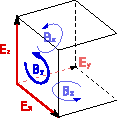
\includegraphics[width=0.4\textwidth]{figures/maggs-rotation}
  \caption{Spatial elements of a cell complex}
  \label{fig:cellstructure}  
\end{figure}

In the implementation of the algorithm we assume that particles with
masses $m_i$ and charges $q_i$ live in the continuum (off--lattice
approach). The charges are interpolated on the lattice with grid
spacing $a$ using a linear interpolation scheme.

\section{Initialization of the algorithm}

The algorithm as it is implemented only calculates stepwise time
updates of the exact field solution. Therefore in order to start the
simulation for the given random distribution of charges we have to
calculate the initial electrostatic field, i.~e. the exact solution of
the electrostatic problem. We find a particular solution of Gauss' law
as the result of the following recursive procedure (see
Fig.~\ref{fig:maggs-initialization}):

\begin{enumerate}
\item The charge in the plane $z=z_\text{plane}$ is
\begin{equation}
  q_\text{plane}=\frac{1}{N_z}\sum_iq(\vec r_i)\delta(z_i-z_\text{plane}),
\end{equation}
$N_z$ is the number of charges in plane $z=z_\text{plane}$. Update the
$z$-field according to the formula
\begin{equation}
  E_z^2=E_z^1+\frac{q_\text{plane}}{\epsilon_0a^2};
\end{equation}
\item Subtract the charge $q_\text{plane}$ from the each charge on
  sites of $z_\text{plane}$. The charge of the wire $y=y_\text{wire},
  z=z_\text{plane}$ is
\begin{equation}
  q_\text{wire}=\frac{1}{N_y}\sum_iq(\vec r_i)\delta(z_i-z_\text{plane})\delta(y_i-y_\text{wire}),
\end{equation}
$N_y$ now meaning the number of charges in the wire. Update $y$-field
\begin{equation}
  E_y^2=E_y^1+\frac{q_\text{wire}}{\epsilon_0a^2};
\end{equation}
\item Subtract the charge $q_\text{wire}$ from the each charge on the
  sites of $(y_\text{wire},z_\text{plane})$. Update $x$ field
\begin{equation}
  E_x^2=E_x^1+\frac{q_\text{vertex}}{\epsilon_0a^2}
\end{equation}
\end{enumerate}

This scheme is repeated until the fields are completely relaxed
(i.~e. the energy is minimized). During repetition, the spatial
dimensions are permutated to avoid a drift in one direction.

\begin{figure}[ht]
  \centering 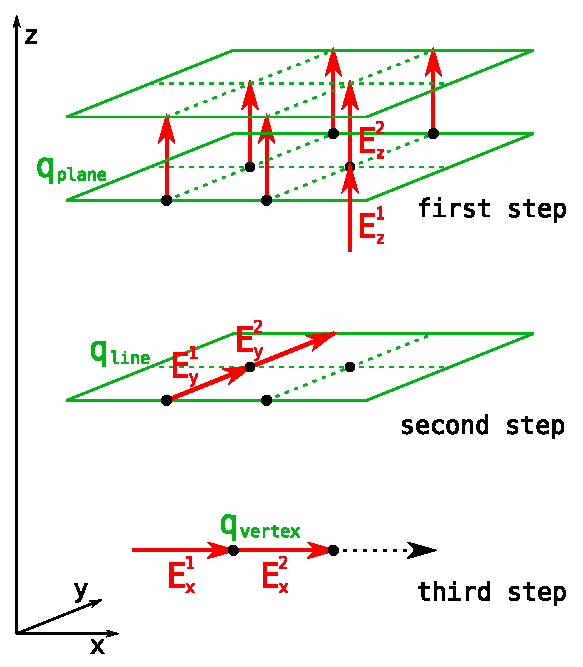
\includegraphics[width=0.4\textwidth]{figures/maggs-initial-scheme}
  \caption{Recursive solution of Gauss' law}
  \label{fig:maggs-initialization}
\end{figure} 

\section{Time integrator}

For the time discretization we have adopted the elegant solution which was found by
Rottler and Maggs \cite{maggs02a} and allows to conserve {\em both}
time--reversibility and phase--space volume conservation:

\begin{enumerate}
\item Update the particle momenta by half a time step.
\item Update the $\vec B$ field by half a time step.
\item Update the particle positions in $x$ direction by half a time
  step.
\item Update the electric field in $x$ direction by half a time step.
\item Update the particle positions in $y$ direction by half a time
  step.
\item Update the electric field in $y$ direction by half a time step.
\item Update the particle positions in $z$ direction by half a time
  step.
\item Update the electric field in $z$ direction by a full time step.
\item Update the particle positions in $z$ direction by half a time
  step.
\item Update the electric field in $y$ direction by half a time step.
\item Update the particle positions in $y$ direction by half a time
  step.
\item Update the electric field in $x$ direction by half a time step.
\item Update the particle positions in $x$ direction by half a time
  step.
\item Update the $\vec B$ field by half a time step.
\item Update the particle momenta by half a time step.
\end{enumerate}

\section{Self--energy}

The interpolation of the charges onto the lattice gives rise to the
artificial force exerted on the particle by its own field. In order to
cure this remedy, the direct subtraction of the self--energy is
introduced.

For the interpolated charge cloud the self--energy can be directly
calculated. For the simple cubic lattice in three dimensions the
linear interpolation will give 8 charges which are placed at the
corners of the cube with edge length $a$ (see
Fig.~\ref{fig:charge-assignment}).

\begin{figure}[ht]
  \centering
  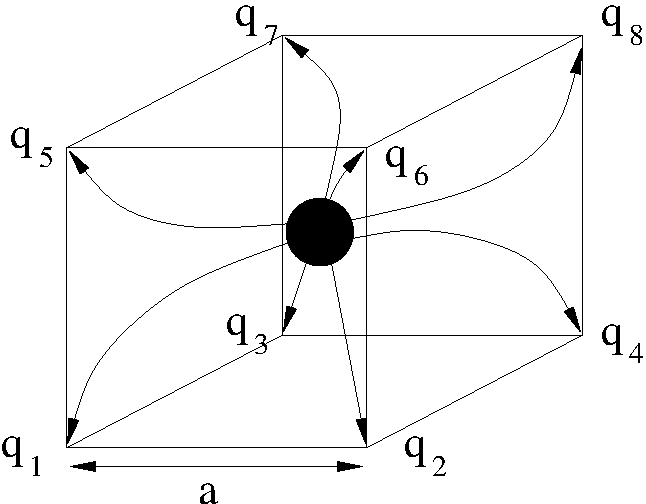
\includegraphics[width=0.3\textwidth]{figures/maggs-charge-assignment}
  \caption{Linear interpolation scheme} 
  \label{fig:charge-assignment}  
\end{figure}

Therefore in our case the self-energy is a symmetric bilinear form
defined by the matrix $\left\{\alpha_{ij}\right\}$, the elements of
which do not depend on the position of the charge. In our algorithm
the values of the coefficients are

\begin{equation}
  \alpha_{ij}=\frac{1}{4a\epsilon_0L^3}\sum\limits_{\vec k}
  \frac{\cos \vec k(\vec R_{\imath}-\vec R_{\jmath})}
  {\sum_{\imath=1}^3(1-\cos\vec k\vec a_{\imath})}
\end{equation}

where $L$ is the number of lattice points per dimension, $\vec R_i$
coordinates of the interpolated charges and $\vec k$ the wave vector.
Those values are calculated during the initialization step and are
used in the calculation of the self-force. The value of the self-force
which has to be subtracted from the overall forces is given by the
following ansatz

\begin{equation}
  \vec F_{self}=-\frac{\partial \mathcal U_{self}}{\partial\vec r}
  =-\sum\limits_i\sum\limits_j\alpha_{ij}
  \left[q_i\frac{\partial q_j}{\partial\vec r}
    +q_j\frac{\partial q_i}{\partial\vec r}\right].
\end{equation}

\section{For which systems to use the algorithm}

Although it is not very well known by now, this algorithm is a
promising alternative to the often used Ewald-based methods. The main
advantages and disadvantages shall be named here. However, it is still
best to understand the concept of the algorithm and figure out for
yourself, if it may be an option.

\begin{itemize}
\item[-] The fields are not calculated for an arbitrary charge
  distribution, but updated from the last solution. Therefore,
  particles should not move too much between timesteps (less than a
  lattice cube).
\item[-] No procedure for error tuning yet. You have to adjust the
  parameters and determine the error yourself.
\item[-] Only 3D periodic systems are possible for now.
\item[-] With the given interpolation scheme, the short-range part of
  the potential is highy underestimated when two particles are in the
  same lattice cube!
\item[-] The initialization routine scales with $\mathcal{O}(N^3)$ and
  takes a long time for larger (and also inhomogenous) systems.
\item[+] The algorithm is a local update scheme and spatially varying
  properties can be applied (in the future).
\item[+] Because of the locality, the algorithm itself scales
  $\mathcal{O}(N)$ and has a big advantage in speed for larger
  systems.
\item[+] Because of the locality, it is highly parallelized.
\item[+] It is fast.
\end{itemize}

The last item is of course dependent on the system properties. But if
the charges are evenly distributed and the system is not too sparse,
this algorithm outperforms P3M easily. Especially for systems with
more than 1000 charges.

Of course, if the system is not dense enough, one will have to set the
lattice spacing in a way to avoid several particles in one cell and
the mesh will be very fine for not so many charges. Also, if you have
lots of charges but your simulation should only run for a short time,
the initialization scheme takes too long in comparison.

But, if you have dense systems with more than 1000 charges or
simulations that run for many timesteps, this method is definitely an
option.
